\section{Verifica}
\label{sez:verifica}

La verifica è una fase cruciale del ciclo di vita del \textit{software}, finalizzata a garantire che il prodotto sviluppato soddisfi i requisiti specificati e sia privo di errori o difetti.\\
Questa attività si concentra sul controllo della correttezza, della completezza e della qualità del \textit{software}, sia a livello di codice che di comportamento.\\

\noindent La verifica può essere suddivisa in due approcci principali:

\begin{itemize}
\item \textbf{Analisi statica}:
È un processo che analizza il \textit{software} senza eseguirlo. \\
Si basa su tecniche di analisi statica, come le revisioni manuali del codice, l'uso di strumenti automatici per il controllo delle regole di codifica o per il \textit{linting} del codice. \\
Questo approccio consente di individuare errori, violazioni di standard, vulnerabilità e problemi di stile a livello di codice sorgente.  

\item \textbf{Analisi dinamica}:
Si basa sull’esecuzione del \textit{software} per testarne il comportamento in ambienti controllati o reali.\\
Questo approccio verifica che il sistema funzioni correttamente con \textit{input} specifici e che produca gli \textit{output} attesi. \\
Include attività come i \textit{test} unitari, \textit{test} di integrazione e \textit{test} di sistema.  
\end{itemize}

\noindent L’utilizzo combinato di analisi statica e dinamica è essenziale per garantire un livello elevato di qualità del \textit{software}. \\
Mentre l'analisi statica permette di affrontare i problemi a monte, l'analisi dinamica assicura che il sistema funzioni correttamente in condizioni operative. \\
Questo approccio integrato riduce al minimo il rischio di errori nel prodotto finale, migliorando l'affidabilità e la robustezza complessiva del \textit{software}.

\subsection{Analisi statica}
\label{subsec:analisi-statica}

L’analisi statica è stata effettuata per garantire che il codice sviluppato fosse conforme agli standard di qualità richiesti, riducendo la possibilità di errori e migliorandone la leggibilità e la manutenibilità.\\
Per questa attività sono stati utilizzati strumenti consolidati come \textit{Prettier} ed \textit{ESLint}, configurati per integrarsi con il flusso di lavoro del progetto.\\

\subsubsection{Utilizzo di Prettier}  
Ho impiegato \textit{Prettier} per il formattamento automatico del codice, con lo scopo di garantire uniformità nello stile e facilitare la leggibilità del codice sorgente.\\
Il formattamento è stato applicato automaticamente durante la fase di sviluppo, tramite l'integrazione con l'\gls{ide} \textit{VSCode}.

\subsubsection{Utilizzo di ESLint}  
Ho utilizzato \textit{ESLint} per individuare e correggere errori di sintassi, violazioni di regole di codifica e possibili \textit{bug} a livello di codice. \\
L’azienda mi ha fornito un loro \textit{setup} di \textit{ESLint}, includendo un insieme di regole e configurazioni specifiche per garantire la conformità agli standard interni.\\
Inoltre, \textit{ESLint} è stato configurato per bloccare il \textit{commit} del codice che non rispettava le regole, garantendo che il codice aggiunto al \textit{repository} fosse sempre conforme alle linee guida aziendali.

\subsection{Analisi dinamica}
\label{subsec:analisi-dinamica}

L’analisi dinamica è stata effettuata per verificare il corretto funzionamento delle diverse componenti del sistema, con un particolare focus sul \gls{backend}, considerato il cuore del progetto, rispetto al \gls{frontend}, il cui \textit{testing} è stato affrontato solo in un secondo momento. \\
Le attività di \textit{testing} si sono concentrate prevalentemente su \textit{test} unitari, con l'aggiunta di alcuni \textit{test} di performance per la generazione dei progetti.\\

\subsubsection{Testing del \gls{backend}}  
Per il \textit{testing} del \gls{backend} è stato utilizzato \textit{Jest}, un \textit{framework} completo e performante per il \textit{testing} in ambiente \textit{JavaScript/TypeScript}.\\
Sono stati sviluppati \textit{test} unitari per tutti i \textit{controller} e i \textit{service}, assicurando la copertura di tutte le principali funzionalità del sistema.\\

\noindent Durante il \textit{testing}:
\begin{itemize}
    \item I \textit{test} sono stati eseguiti durante tutto il ciclo di vita del \textit{software}, seguendo il modello a \textit{V} (visibile in {\hyperref[fig:v-model]{Figura 3.8}}), che prevede l’integrazione di attività di \textit{testing} in ogni fase di sviluppo.\\
    Man mano che venivano creati gli \textit{endpoint}, sono stati sviluppati i relativi \textit{test} per verificarne immediatamente la correttezza;
    \item Sono stati creati \textit{mock} delle entità per simulare i dati e isolare le singole componenti testate, garantendo che i \textit{test} non dipendessero da altre parti del sistema;
    \item Per la generazione dei progetti, è stato sviluppato un \textit{mockup} di \textit{LangChain}, consentendo di verificare il corretto flusso di dati e la validità del processo di generazione senza richiedere chiamate ad \gls{llm};
    \item Per il salvataggio dei PDF, è stato implementato un \textit{mockup} del servizio \textit{AWS S3}, simulando le operazioni di caricamento e verifica dei \textit{file} per testare l’interazione con il servizio senza dipendere da risorse esterne.
\end{itemize}

\noindent Questo approccio iterativo ha garantito che ogni componente fosse testata e verificata fin dalla sua creazione, riducendo al minimo la possibilità di accumulare errori e semplificando il \textit{debug} nelle fasi successive.\\

\begin{figure}[H]
    \centering
    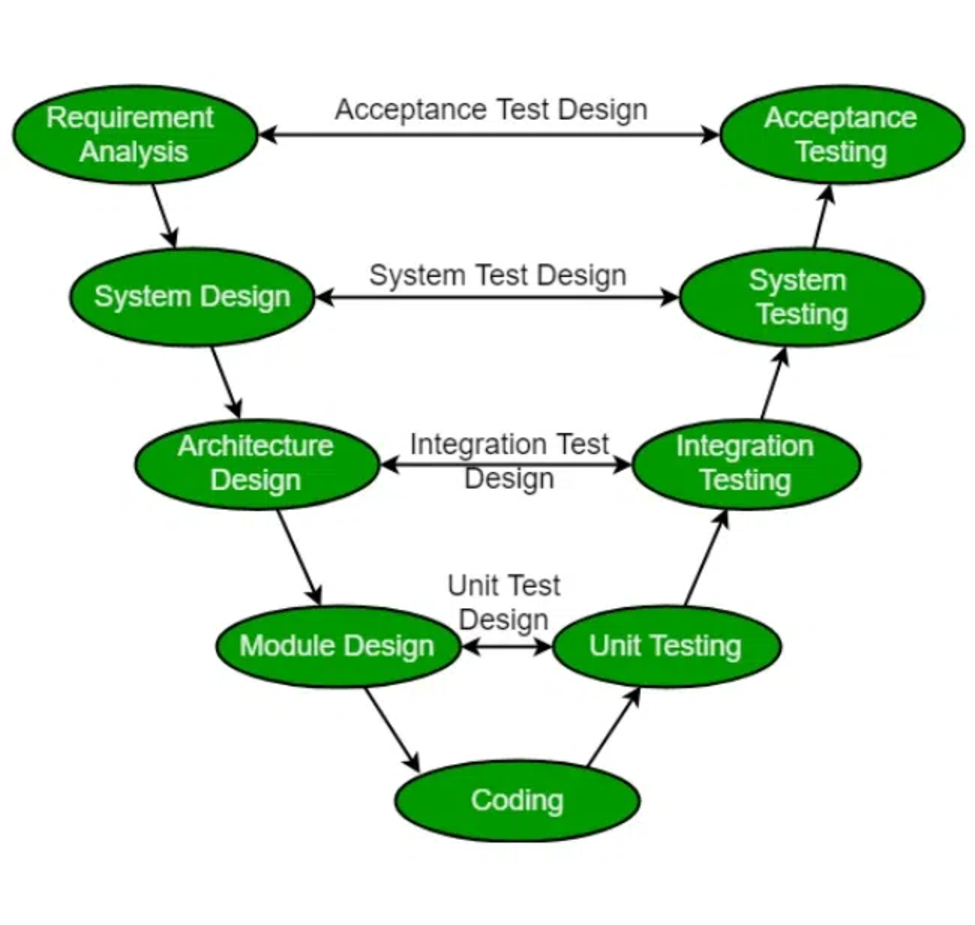
\includegraphics[scale=0.43]{v-model.png}
    \caption{Modello a V}
    \label{fig:v-model}  
    \cite{site:v-model}
\end{figure}

\subsubsection{Testing del \gls{frontend}}  
Il \textit{testing} del \gls{frontend} è stato affrontato in una fase successiva rispetto al \gls{backend}, con un approccio più limitato.\\
Le attività principali si sono concentrate sulla verifica manuale delle interfacce utente e sull’esecuzione di \textit{test} funzionali di base per garantire che le interazioni principali fossero fluide e prive di errori.\\
Sono stati implementati alcuni \textit{test} di unità per i componenti \textit{React} più complessi, utilizzando \textit{React Testing Library} per simulare le interazioni dell'utente e verificare il corretto funzionamento dei componenti.\\

\subsubsection{Test di performance}  
Sono stati effettuati alcuni \textit{test} di performance specifici per il \gls{backend}, con un focus particolare sulla generazione dei progetti.\\
Questi \textit{test} hanno permesso di misurare i tempi di risposta e verificare che il sistema fosse in grado di gestire la generazione di progetti in modo efficiente, anche in scenari di carico moderato.\\

\noindent L’adozione di un approccio mirato, con particolare attenzione al \textit{testing} del \textit{backend}, all’uso di \textit{mockup} per simulare le dipendenze e all’integrazione continua dei \textit{test}, ha garantito una validazione robusta delle principali funzionalità del sistema, assicurando affidabilità e consistenza nel comportamento delle componenti chiave.